\chapter{Coordinate Geometry}
\setcounter{exercisecounter}{0}

\setcounter{thmcounter}{1}
\section{Introduction}
Many of you have encountered some form of coordinate geometry in high school. For instance, the ``standard" way to visualize a graph e.g. $f(x)=x^2$ is to visualize the points in 2-D space $(x,y)$ where $y=x^2$. We give an demonstration in Python code.

\begin{lstlisting}[language=Python]
import matplotlib.pyplot as plt
import numpy as np
X=np.arange(-100,100) #create list of numbers from -100 to 100
Y= X**2 #calculate the square of at each x
plt.plot(X,Y) #plot all the pairs of points in 2d plane
plt.xlabel('x')
plt.ylabel('y=x^2')
plt.title('Visualization of the "object"')
plt.show()
plt.show()
\end{lstlisting}
\begin{tikzpicture}
	\node (A) at (0,0) {$x$};
	\node (B) at (3,0) {$x^2$};
	\draw[->,thick]
	(A)--(B)
	node[midway,below] {the "graph" object} ;
	\node(whitehead) at (8,0){
		\includegraphics[width=0.6\textwidth]{coordinate_geometry/square_graph.png}
	};
\end{tikzpicture}


This is also known as the Cartesian plane, after Descartes who invented it in the 17th century.\\
\section{Visualization of geometric objects}
The Cartesian plane allows us to describe shapes with equations and perform calculations with them. We first define the playing field (the Cartesian plane and higher dimensional analogues) and the players.
\definition{Real numbers}{
	The set of \textbf{real numbers}, denoted as $\mathbb{R}$, is (informally) the set of all the numbers that can be written out in decimal form.
}
\example{
The following are real numbers:
\begin{enumerate}
	\item The integers $0$, $\pm 1$, $\pm 2$, ...  
	\item Fractions in the form $\frac{a}{b}$, where $a$ and $b\neq 0$ are integers.
	\item Irrational numbers $\sqrt{2}$, $\pi$.
\end{enumerate}
}
\begin{remark}
	The set of real numbers is known as a \textbf{complete field}. The definition of a complete field will be swept under the rug, but it guarantees a few things. The most important property: We will not "escape" the set by performing operations, possibly infinitely many.
\end{remark}
\definition{N-dimensional space}{
	Let $n$ be a positive integer. We denote the \textbf{n-dimensional real space} to be $\mathbb{R}^n$, consisting of all the $n$-tuples $(x_1,x_2,x_3,...,x_n)$, where each $x_j$ is a real number. \\
	We call an $n$-tuple $(x_1,...,x_n)$ a \textbf{point}, and two points $(x_1,...,x_n)$ and $(y_1,...,y_n)$ are equal if $x_j=y_j$ for all $j$-th entries of the tuples.
}
\begin{remark}
	We sometimes use $\mathbf{x}$ to denote $(x_1,...,x_n)$ to make notation cleaner.
\end{remark}
\subsection{Lines}
Now that we have introduced the playing field of n-dimensional space, we can start translating the axioms of euclidean geometry to this coordinate system.
\definition{Lines}{
	In euclidean geometry, a line is defined by two points. We let $\mathbf{x},\mathbf{y} \in \mathbb{R}^n$. The \textbf{line} going from $\mathbf{x}$ to $\mathbf{y}$ is denoted $\overrightarrow{\mathbf{xy}}$.
}
What would this line look like? To get from $\mathbf{x}$ to $\mathbf{y}$, we have to traverse $y_1-x_1$ units in the first coordinate, $y_2-x_2$ units in the second, ..., $y_n-x_n$ in the last. We thus have a natural notation for the line $\overrightarrow{\mathbf{xy}}$.
\[
 \overrightarrow{\mathbf{xy}}=(y_1-x_1,y_2-x_2,...,y_n-x_n).
\]

This is very similar to a point as an n-tuple, but this is "spiritually" different to a point. This tuple represents the direction of line. One way to think of the correspondence between $(x_1,...,x_n)$ point and $(x_1,...,x_n)$ line is that $(x_1,...,x_n)$ line is the line connecting $(0,0,...0)$ to $(x_1,...,x_n)$ point. Because of this, we can identify a tuple as both the point and the line, and we call it a "vector" to abstract away from the actual geometric meaning.
\begin{figure}
	\centering
	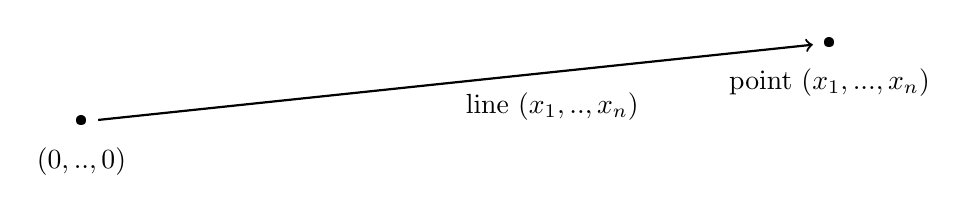
\begin{tikzpicture}[node distance=2cm]
		\node (A)[draw=none,label=below:{$(0,..,0)$}] at (0,0) {\textbullet};
		\node (B)[draw=none,label=below:{point $(x_1,...,x_n)$}] at (9.5,1) {\textbullet};
		
		\draw[thick, ->]
		(A) -- (B) 
		node[midway, below right] {line $(x_1,..,x_n)$};
	\end{tikzpicture}
\end{figure}


\subsection{Operation with lines}
We need to translate a few more things from euclidean geometry.

\proposition{
Let $\mathbf{x}, \mathbf{y}, \mathbf{z} \in \mathbb{R}^n$, then \[
	\overrightarrow{\mathbf{xy}}+\overrightarrow{\mathbf{yz}}=\overrightarrow{\mathbf{xz}},
\]
where $(a_1,...,a_n)+(b_1,...,b_n)\defeq(a_1+b_1,..., a_n+b_n)$.
}
\begin{proof}
	\begin{align*}
		\overrightarrow{\mathbf{xy}}+\overrightarrow{\mathbf{yz}}&=(y_1-x_1,..., y_1-x_n)+(z_1-y_1,..., z_1-y_n)\\
		&=(y_1-x_1+z_1-y_1, ... ,y_n-x_n+z_n-y_n)\\
		&= (z_1-x_1, ...,z_n-x_n)\\
		&= \overrightarrow{\mathbf{xz}}
	\end{align*}
\end{proof}
\

Geometrically, this means if you connect $\mathbf{x}$ to $\mathbf{y}$ to $\mathbf{z}$, the overall "direction of travel" you make is $\mathbf{x}$ to $\mathbf{z}$. This gives us a natural extension for addition of vectors by considering each entry. Similarly for scaling vectors, we just scale the entries along each dimension.

 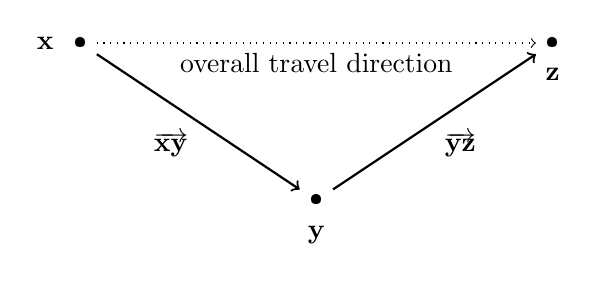
\begin{tikzpicture}[node distance=2cm]
 	\node (A)[draw=none,label=left:$\mathbf{x}$] at (0,0) {\textbullet};
 	\node (B)[draw=none,label=below:$\mathbf{y}$] at (3,-2) {\textbullet};
 	\node (C)[draw=none,label=below:$\mathbf{z}$] at (6,0) {\textbullet};
 
 	\draw[thick, ->]
 	(A) -- (B)
 	node[midway, below left]{$\overrightarrow{\mathbf{xy}}$};
 	\draw[thick, ->]
 	(B) -- (C)
 	node[midway, below right]{$\overrightarrow{\mathbf{yz}}$};
 	
 	\draw[dotted,->]
 	(A)--(C)
 	node[midway, below] {overall travel direction};
 	
 \end{tikzpicture}\ \\

\definition{Addition and scaling of vectors}{
	Let $\vec{a},\vec{b}$ be two vectors in $\mathbb{R}^n$. We define the sum/difference of $\vec{a}$ and $\vec{b}$ \[
		\vec{a}+\vec{b} \defeq (a_1+b_1,...,a_n+b_n), \quad \vec{a}-\vec{b} \defeq (a_1-b_1,...,a_n-b_n)
	\] and the scaling of $\vec{a}$ by a real number $c\in \mathbb{R}$ \[
		c\vec{a} \defeq (c a_1, c a_2,... ,c a_n).
	\]
}
\begin{remark}
	Here we use the term "vectors", as we can in essence add points and lines together. How does one make sense of adding a line to a point? We can view this as translating the point along the path of the line, for instance, let us translate the point $(1,2)$ $3$ units in the first coordinate and $-1$ units in the second coordinate. This will give us $(4,1)$.
 	\textbf{TODO: ADD GRAPH}
\end{remark}
This way, we can write the line from $\vec{x}$ to $\vec{y}$ as $\vec{y}-\vec{x}$. The proof is a computational exercise. \\ 
\begin{notation}
	We now transferred for talking about points and the lines between points to addition. Therefore, we can overload the notation for points and lines as a vector $\vec{v}$, keeping in mind that they have the same arithmetic structure.
\end{notation}


In fact, most of our intuition for the real numbers translate to $\mathbb{R}$. For formality, we will list them here; in practice, we (almost always) take these properties for granted.
\proposition{
	Let $\vec{u},\vec{v},\vec{w} \in \mathbb{R}^n$, and $a,b \in \mathbb{R}$. Then the following hold:
	\begin{itemize}
		\item \textit{(Associativity)} $(\vec{u}+\vec{v})+\vec{w} = \vec{u}+(\vec{v}+\vec{w})$.
		\item \textit{(Commutativity)} $\vec{u}+\vec{v} = \vec{v}+\vec{u}$.
		\item \textit{(Identity)} The zero vector $\vec{0}\defeq (0,0,...,0)\in\reals$ satisfies $\vec{v}+\vec{0}=\vec{v}$.
		\item \textit{(Inverse)} The inverse of $\vec{v}$, $-\vec{v}\defeq(-v_1,...,-v_n)$ satisfies $\vec{v}+(-\vec{v})=\vec{0}$.
		\item \textit{(Scalar multiplication)} $a(b\vec{v})=(ab)\vec{v}$.
		\item \textit{(Scalar Identity)} $1\vec{v}=\vec{v}$.
		\item \textit{(Distributivity 1)}  $a(\vec{u}+\vec{v})=a\vec{u}+a\vec{v}$.
		\item \textit{(Distributivity 2)}  $(a+b)\vec{v}=a\vec{v}+b\vec{v}$.
	\end{itemize}
} 
\begin{remark}
	All of these have good geometric intuition behind. For instance, the zero vector $\vec{0}$ is the ``don't move" vector, corresponding to the point at the origin, or the ``too short to be line''. The inverse of $\overrightarrow{\mathbf{xy}}$ is $\overrightarrow{\mathbf{yx}}$, where you go back from $\mathbf{x}$ to $\mathbf{y}$. \begin{tikzpicture}
		
	\end{tikzpicture}
\end{remark}
\begin{remark}
	These $8$ conditions are the axioms of a vector space. Later in the course, we will generalize the notion of vectors in $\reals^n$ to other spaces (playing fields).
\end{remark}
\proposition{
	Lines are translation invariant. That is, for every $\vec{x},\vec{y},\vec{v}\in\mathbb{R}^n$, then the 
	line from $\vec{x}$ to $\vec{y}$ is the same as the line from $\vec{x}+\vec{v}$ to $\vec{y}+\vec{v}$.
}
Let us illustrate what this statement is trying to convey. We have two points $\vec{x}$, $\vec{y}$; now we translate each of these points by $\vec{v}$, and we want the line between the points to be preserved under this translation.\\
\begin{tikzpicture}
	\node (X)[draw=none,label=left:$\vec{x}$] at (0,0) {\textbullet};
	\node (Y)[draw=none,label=below:$\vec{y}$] at (5,-1) {\textbullet};
	\node (XT)[draw=none,label=below:$\vec{x}+\vec{v}$] at (-2,-2) {\textbullet};
	\node (YT)[draw=none,label=below:$\vec{y}+\vec{v}$] at (3,-3) {\textbullet};
	
	\draw[->,thick] 
	(X)--(Y)
	node (a)[midway, above right] {$\vec{y}-\vec{x}$};
	
	\draw[->,dotted] 
	(X)--(XT)
	node[midway, above left] {$\vec{v}$};
	
	\draw[->,dotted] 
	(Y)--(YT)
	node[midway, above left] {$\vec{v}$};
	
	
	\draw[->,color=blue] 
	(XT)--(YT)
	node[midway, below left] {?};
\end{tikzpicture} \ \\
The proof is one line: $(\vec{y}+\vec{v}) - (\vec{y}+\vec{v}) = \vec{y}-\vec{x} +\vec{v}-\vec{v}=\vec{y}-\vec{x}$. However, an immediate consequence of this is that we can ``transport'' vectors in space without distorting the vector. Colloquially, \textit{5 miles South} to you describes the same direction and length as \textit{5 miles South} to a person a few feet away. This justifies the way we visualize the correspondence between points and vectors - we ``transport'' the vectors to start from the origin $(0,...,0)$, and the end describes the point.

\begin{remark}
	Translation (and scaling) invariance is a property of Euclidean geometry. There are some exotic geometry systems that distort distance and direction through translation and scaling. One such example is the Poincar\'e metric.
\end{remark}
Another notion we can carry from Euclidean geometry is parallel lines. Here we not only define what it means for two vectors to be parallel (never touching), we also give a definition for two vectors to be parallel but point in opposite directions.
\definition{Parallel and Antiparallel Vectors}{
	Let non-zero vectors $\vec{v},\vec{w}\in\reals^n$.
	We say that $\vec{v}$ and $\vec{w}$ are \textbf{parallel} if there is some $c>0$ such that $\vec{v}=c\vec{w}$. We say that $\vec{v}$ and $\vec{w}$ are \textbf{antiparallel} if there is some $c<0$ such that $\vec{v}=c\vec{w}$.
}
%
Finally, the nice algebraic properties for adding and scaling vectors gives us a natural way to understand these vectors as a sum of $n$ component vectors, one for each dimension. These \textit{special} vectors deserve a name.
\definition{Standard Basis Vectors and Vector Decomposition}{
	We denote in $\reals^n$, the \textbf{standard basis vectors} \begin{align*}
		\vec{e}_1 &\defeq (1,0,0,...,0,0,0),\\
		\vec{e}_2 &\defeq (0,1,0,...,0,0,0),\\
		\vec{e}_{n-1}&\defeq (0,0,0,...,0,1,0),\\
		\vec{e}_n&\defeq(0,0,0,...,0,0,1),
	\end{align*}
	so that $\vec{v}=\sum_{i=1}^n v_i \vec{e}_i$.
	In $\reals^3$, we sometimes write \[
		\vec{i}\defeq \vec{e}_1, \quad \vec{j}\defeq \vec{e}_2,\quad \vec{k}\defeq\vec{e}_3
	\]to accommodate the physicists.
}\ \\
\exercises
\begin{exerciselist}
	\item Compute $5\vec{v}-2\vec{w}$ and $-3\vec{w}$ for the following pairs of vectors: \begin{enumerate}[label=(\alph*)]
		\item $\vec{v}=2\vec{i}+3\vec{j}$, $\vec{w}=4\vec{i}-9\vec{j}$
		\item $\vec{v}=(1,2,-1)$, $\vec{w}=(2,-1,0)$
		\item $\vec{v}=-2\vec{e}_3+4\vec{e}_5$, $\vec{w}=\vec{e}_1 -4\vec{e}_5$
		\item $\vec{v}=(\cos t, \sin t)$, $\vec{w}=(\cos t)\vec{e}_2 - (\sin t) \vec{e}_1$
	\end{enumerate}
	\item Find the vector $\overrightarrow{PQ}$ connecting $P(7,2,9)$ to $Q(-2,1,4)$. Put your answer in the form $a\vec{i}+b\vec{j}+c\vec{k}$.
\end{exerciselist}
\section{Length, angles and projections}
\definition{Magnitude}{
Let $\vec{v}\in\reals^n$. The magnitude of $\vec{v}$ is denoted \[
|\vec{v}| \defeq \sqrt{v_1^2 + v_2 ^2+ ... v_n^2}.
\]
}
We build intuition through the lower dimensional cases.
In $\reals^2$, let us consider the point $(4,3)$.\\
\begin{wrapfigure}{r}{0.3\textwidth}
	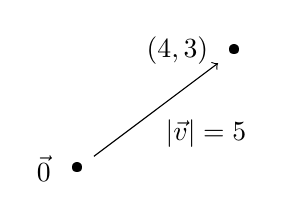
\begin{tikzpicture}
		\node (X)[draw=none,label=left:{$\vec{0}$}] at (0,0) {\textbullet};
		\node (Y)[draw=none,label=left:{$(4,3)$}] at (2,1.5) {\textbullet};
		\draw[->]
		(X)--(Y)
		node [midway, below right] {$|\vec{v}|=5$};
	\end{tikzpicture}
\end{wrapfigure}

The magnitude of this vector is $\sqrt{3^2+4^2}=5$. If this sounds very familiar, it is because this is indeed an application of Pythagorean theorem. In 3-dimensions, this still applies - take $\vec{x}=(a,b,c)$, we can traverse in each coordinate to apply Pythagorean theorem twice.

\usetikzlibrary {3d}

\begin{figure}
	\centering
	\begin{tikzpicture}
		
		\draw[->](0,0,0) -- (xyz cylindrical cs:radius=3);
		\node at (3.5,0,0){$x_1$};
		\draw[->] (0,0,0) -- (xyz cylindrical cs:radius=3,angle=90);
		\node at (0,3.5,0){$x_2$};
		\draw[->] (0,0,0) -- (xyz cylindrical cs:z=3);
		\node at (0,0,3.5){$x_3$};
		\draw[->,dotted,thick,color=red] (0,0,0) -- (2,0,0)
		node[midway,below]{a};
		\draw[->,dotted,thick,color=red] (2,0,0) -- (2,3,0) node[midway,right]{b};
		\draw[->,dotted,thick,color=red] (2,3,0) -- (2,3,1)
		node[midway,above]{c};
		\draw[->,color=blue] 
		(0,0,0) -- (2,3,1)
		node[midway, below]{$\vec{x}$};
	\end{tikzpicture}
	\centering
	\begin{tikzpicture}
		
		\draw[->](0,0,0) -- (xyz cylindrical cs:radius=3);
		\node at (3.5,0,0){$x_1$};
		\draw[->] (0,0,0) -- (xyz cylindrical cs:radius=3,angle=90);
		\node at (0,3.5,0){$x_2$};
		\draw[->] (0,0,0) -- (xyz cylindrical cs:z=3);
		\node at (0,0,3.5){$x_3$};
		\draw[->,dotted,thick,color=red] (0,0,0) -- (2,0,0)
		node[midway,below]{a};
		\draw[->,dotted,thick,color=red] (2,0,0) -- (2,3,0) node[midway,right]{b};
		\draw[->,color=brown] 
		(0,0,0) -- (2,3,0)
		node[midway, left]{$\sqrt{a^2+b^2}$};
		
	\end{tikzpicture}
	\centering
	\begin{tikzpicture}
		[z={(10:10mm)},x={(-45:5mm)}]
		
		\draw[->](0,0,0) -- (3,0,0);
		\node at (3.5,0,0){$x_1$};
		\draw[->] (0,0,0) -- (0,3,0);
		\node at (0,3.5,0){$x_2$};
		\draw[->] (0,0,0) -- (0,0,-3);
		\node at (0,0,-3.5){$x_3$};
		\draw[->,color=brown] 
		(0,0,0) -- (2,3,0)
		node[midway, right]{$\sqrt{a^2+b^2}$};
		
		\draw[->,dotted,thick,color=red] (2,3,0) -- (2,3,-1) node[midway, above]{c};
		\draw[->,color=blue] 
		(0,0,0) -- (2,3,-1)
		node[midway, left]{$\sqrt{a^2+b^2+c^2}$};
	
	\end{tikzpicture}
\end{figure}\ \\

\proposition{
	Let $\vec{v} \in \reals^n, a\in\reals$. Then \[
	|a\vec{v}| = |a||\vec{v}|.
	\]
}\ \\
We have now transported the notions of length and scaling into the coordinate system, and this allows us to make ``measurements'' such as angles and area.

\subsection{The Dot Product}
\example{
Let points A=$(5,8)$, B=$(-2, 7)$, O=$(4,5)$. Find the angle $\angle AOB$.
}
To solve this using only information about the lengths, recall the Law of Cosines:

\theorem{Law of Cosines}{
For any triangle 
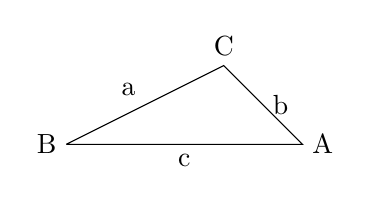
\begin{tikzpicture}
	
	\draw (0,0) node [left] {B}--(2,1) node [above]{C} node [midway, above left]{a}--(3,0) node [right]{A} node [midway, right]{b}--(0,0)node [midway, below]{c};
	%pic["$\alpha$",draw=orange,<->,angle eccentricity=1.2,angle radius=1cm] {angle=(0,0)--(2,1)--(3,0)};
\end{tikzpicture},
\[
	c^2 = a^2+b^2 - 2 a b \cos(\angle BCA).
\]
}

We now apply the Law of Cosines to $\triangle AOB$, so that\[
	|\overrightarrow{AO}|^2  +|\overrightarrow{OB}|^2- 2 |\overrightarrow{AO}| |\overrightarrow{OB} \ |\cos(\angle AOB) = |\overrightarrow{AB}|^2.
\]
Plugging in the values, we solve 
\begin{align*}
		((4-5)^2 + (5-8)^2) + ((-2-4)^2+(7-5)^2) - 2 \sqrt{(4-5)^2 + (5-8)^2} \\ \times \sqrt{(-2-4)^2+(7-5)^2} \cos(\angle AOB) = ((-2-5)^2+(7-8)^2).
\end{align*}
Simplifying, we get\[
	50 - 2 \sqrt{10} \sqrt{40} \cos(\angle AOB) = 50 \implies \cos(\angle AOB) = 0.
\]
So the angle is $\pi/2$.

\example{
	Find a closed form formula for the cosine of an angle formed by two vectors $\vec{v},\vec{w} \in\reals^n$.
}
Let the angle formed be $\theta$. Using the intuition from 2-D space, we can form a triangle (in a very complex n-dimensional space). We write the Law of Cosine in terms of vectors
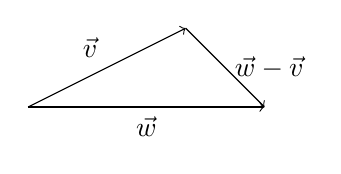
\begin{tikzpicture}
	
	\draw [->](0,0) -- (2,1) node [midway, above left]{$\vec{v}$};
	\draw [->](0,0)--(3,0) node [midway, below]{$\vec{w}$};
	\draw [->](2,1)--(3,0)node [midway, right]{$\vec{w}-\vec{v}$};
	%pic["$\alpha$",draw=orange,<->,angle eccentricity=1.2,angle radius=1cm] {angle=(0,0)--(2,1)--(3,0)};
\end{tikzpicture}
 \[
|\vec{v}|^2+|\vec{w}|^2-2|\vec{v}||\vec{w}|= |\vec{w}-\vec{v}|^2.
\]
This expands to \begin{align*}
	\sum_{i=1}^{n} v_i^2 + \sum_{j=1}^{n} w_j^2  - 2 \sqrt{\sum_{i=1}^{n} v_i^2}\sqrt{\sum_{j=1}^{n} w_j^2} \ \cos(\theta) =
	\sum_{i=1}^n (w_i-v_i)^2.
\end{align*}
Rearranging $(a-b)^2 = a^2+b^2-2ab$,
\[
2 \sqrt{\sum_{i=1}^{n} v_i^2}\sqrt{\sum_{j=1}^{n} w_j^2} \ \cos(\theta) = \sum_{i=1}^n 2 w_i v_i 
\]
so \[
\cos(\theta) = \frac{\sum_{i=1}^n w_i v_i }{\sqrt{\sum_{i=1}^{n} v_i^2}\sqrt{\sum_{j=1}^{n} w_j^2}}.
\]
\definition{Dot Product}{
	Let $\vec{v},\vec{w}\in\reals^n$, the \textbf{dot product} between $\vec{v}$ and $\vec{w}$ is \[
		\vec{v} \cdot \vec{w} \defeq \sum_{i=1}^n v_i w_i. 
	\]
}
\proposition{
	Let $\vec{u},\vec{v},\vec{w}\in\reals^n$, $c\in\reals$. The dot product satisfies the following properties:
	\begin{itemize}
		\item \textit{(Symmetry)} $\vec{v}\cdot\vec{w}=\vec{w}\cdot\vec{v}$.
		\item \textit{(Linearity 1)} $(c\vec{v})\cdot\vec{w} = c (\vec{v}\cdot\vec{w}) \textrm{(}= \vec{v}\cdot(c\vec{w})\textrm{  by symmetry)}$.
		\item \textit{(Linearity 2)} $(\vec{v}+\vec{u})\cdot\vec{w} = \vec{v}\cdot\vec{w}+\vec{u}\cdot\vec{w}$.
		\item \textit{(Positive definiteness)} $\vec{v} \cdot\vec{v}\geq0$, with equality if and only if $\vec{v}=\vec{0}$.
	\end{itemize}
}
\begin{proof}
	\textbf{TODO: write the proof, or put it as an exercise.}
\end{proof}
\corollary{
	
	\begin{enumerate}
		\item $
		|\vec{v}-\vec{w}|^2 = |\vec{v}|^2 + |\vec{w}|^2 - 2 \vec{v}\cdot\vec{w}.
		$
		\item If $\vec{v},\vec{w}\neq \vec{0}$, the angle between $\vec{v}$ and $\vec{w}$ is\[
		\cos^{-1}\left(\frac{\vec{v}\cdot\vec{w}}{|\vec{v}||\vec{w}|}\right).
		\]
		In particular, the angle is $\pi/2$ when $\vec{v}\cdot\vec{w}=0$. 
		\item $|\vec{v}\cdot\vec{w}|\leq |\vec{v}||\vec{w}|.$
	\end{enumerate}
}\label{dotproductcor}
Since we can make sense of ``angles'' in higher dimensions, it is natural to generalize the notion of two vectors ``perpendicular'' to each other.
\definition{Orthogonality}{
Let $\vec{v},\vec{w}\in\reals^n$. We say $\vec{v}$ and $\vec{w}$ are \textbf{orthogonal} to each other if $\vec{v}\cdot\vec{w}=0$.
}

\example{
	Find all vectors $\vec{v}\in\reals^3$ such that $\vec{v}\cdot(-3\vec{i}+2\vec{j}+6\vec{k}) =49$. Sketch the locus of corresponding points in $\reals^3$.
}\label{plane_projection}
The condition expands to \begin{align*}
	-3v_1+2v_2+6v_3 &= 49 \\
	\implies v_3 &= \frac{49+3v_1 - 2v_2}{6}  
\end{align*}
so that the set of all vectors is \[
	\left\{s \vec{i}+t \vec{j}+\left(\frac{49+3s - 2t}{6}\right) \vec{k} | s,t\in\reals\right\}.
\]
To plot this in 3D space, notice that this describes the equation of a plane $z={(49+3x-2y)}/{6}$. We pick any three points (of course we want those that are easy to calculate) $(0,0,49/6)$, $(0,49/12,0)$, $(-49/18,0,0)$.
\iffalse
\begin{figure}
	\centering

	\subfloat%[\centering label 1]
	{{\includegraphics[width=7cm]{coordinate_geometry/plane1.png} }}%
	\qquad
	\subfloat%[\centering label 2]
	{{\includegraphics[width=7cm]{coordinate_geometry/plane2.png} }}%
	\caption{Two views of the plane}
\end{figure}
\fi
\begin{figure}
	\centering
	\includegraphics[width=\textwidth]{coordinate_geometry/plane2.png}
	\caption{Two views of the plane}
\end{figure}\ \\

Interestingly, we see that $(-3,2,6)$ - the point corresponding to our vector - is a point on the plane!

\subsection{Projection}
\definition{Projection}{
Let $\vec{v},\vec{w}\in\reals^n$, $\vec{v}\neq\vec{0}$, and $c\in\reals$, such that $\vec{v}\cdot(\vec{w}-c\vec{v})=0$ (or equivalently, $\vec{w}-c\vec{v}$ orthogonal to $\vec{v}$). 

We say that $c\vec{v}\defeq \textrm{Proj}_{\vec{v}} (\vec{w})$ is the \textbf{vector projection of $\vec{w}$ on $\vec{v}$}.

}\ \\

\iffalse
\begin{notation}
	The vector projection ``encodes'' information about the scalar projection. Therefore, if we do not specify scalar or vector, assume are talking about vector projections.
\end{notation}
\fi
To build intuition, it is always helpful to start with lower dimensions. We take a plane through $\vec{v}$ and $\vec{w}$. Looking at this slice, we can work in 2D.

	
\begin{tikzpicture}
		\node (A) at (0,0) {TODO};
	\end{tikzpicture}
	
	

We see that $c\vec{v}$ is the the point on the extension of $\vec{v}$ such that it is closest to the point $\vec{w}$. To geometrically show this idea, we draw a circle centered at $\vec{w}$ with radius $|\vec{w}-c\vec{v}|$. The line generated by $\vec{v}$ is tangent to this circle, so the contact point at $c\vec{v}$ is indeed the closest point to $\vec{w}$. 

We also see from this geometric construction that 1) the projection $c\vec{v}$ is unique thus well defined, 2) $c|\vec{v}|=|\vec{w}|\cos \theta$

\proposition{
The projection is unique and is given by \[
	\textrm{Proj}_{\vec{v}}(\vec{w}) = \frac{\cos \theta |\vec{w}|}{|\vec{v}|} = \frac{\vec{v}\cdot\vec{w}}{|\vec{v}|^2} = (\frac{\vec{v}\cdot\vec{w}}{\vec{v}\cdot\vec{v}})\vec{v}.
\]

}
This is the first time we show that something is unique. The standard argument goes as follows: Suppose another object $a'$ satisfies all the properties you want for $a$. Then you can show $a=a'$, meaning every object that satisfies the properties is $a$, or equivalently, $a$ is unique. 

So what happens if we pick two points $P$, $P'$ on $\vec{v}$ such that both make a right angle when connected to $\vec{w}$? We would have constructed a triangle $\triangle PP'\vec{w}$ with two right angles!
\begin{proof}
	Let $c, c'\in\reals$ such that $\vec{p}_1=c\vec{v}$ and $\vec{p}_2=c'\vec{v}$ are both satisfy the definition of $\textrm{Proj}_{\vec{v}}({\vec{w}})$. We want to show that $c=c'$, so we consider $\vec{u}=(c-c')\vec{v}$, the line between the two projections.\\
	By a corollary in \ref{dotproductcor}, we have two equations \begin{align*}
	|\vec{w}-\vec{p}_1|^2&=|\vec{w}-\vec{p}_2|^2+|\vec{u}|^2 \\	
	|\vec{w}-\vec{p}_2|^2&=|\vec{w}-\vec{p}_1|^2+|\vec{u}|^2 
	\end{align*}
	We can solve for $|\vec{u}|=0$, and by positive definiteness, $\vec{u}=\vec{0}$ and $c-c' = |\vec{u}|/|\vec{v}| =0$.\\
	To show our formula for projection works, we can just compute that \[
	\vec{v} \cdot \left(\vec{w}-\left(\frac{\vec{v}\cdot{\vec{w}}}{\vec{v}\cdot\vec{v}}\right)\vec{v}\right)=\vec{v}\cdot\vec{w} -\left(\frac{\vec{v}\cdot\vec{w}}{\vec{v}\cdot\vec{v}}\right)(\vec{v}\cdot\vec{v})=0.
	\]
\end{proof}
\exercises
\begin{exerciselist}
	\item Determine if the following pairs of vectors are orthogonal: \begin{enumerate}[label=(\alph*)]
		\item $3\vec{e}_1+4\vec{e}_2$, $-4\vec{e}_1+3\vec{e}_2$
		\item $(4,-1,2)$, $(3,0,-6)$
		\item $3\vec{i}-2\vec{j}$, $-2\vec{i}-4\vec{k}$
		\item $\vec{e}_1 + 3\vec{e}_3 + 5\vec{e}_5+ ...+(2k-1)\vec{e}_{2k-1}$, $2\vec{e}_2+4\vec{e}_4+...+(2k)\vec{e}_{2k}$
	\end{enumerate}
	\item Refer to the plane in the example in the previous section \ref{dotproductcor}. Show that $\textrm{Proj}_{-3\vec{i}+2\vec{j}+6\vec{k}}(\vec{v})$ is the same for any vector $\vec{v}$ such that $\vec{v}\cdot(-3\vec{i}+2\vec{j}+6\vec{k}) =49$, and compute this projection.
	\item \textit{(Geometry of a methane molecule)} Place four points $P(0,0,0)$, $Q(1,1,0)$, $R(1,0,1)$, $S(0,1,1)$ in $\reals^3$. \begin{enumerate}[label=(\alph*)]
		\item Compute the distance between any two points of $PQRS$ and show that all $6$ pairs are the same. This means that $PQRS$ forms a regular tetrahedron.
		\item  Verify that the geometric center of the tetrahedron $O(1/2, 1/2, 1/2)$ is equidistant to all of the vertices of the tetrahedron.
		\item Compute the angle between two edges of the tetrahedron, rounded to $2$ decimal places. By symmetry, you only have to compute one angle.
		\item Compute the angle $\angle POQ$, rounded to $2$ decimal places. Does this angle remind you of something from Chemistry?
	\end{enumerate}
\end{exerciselist}
\section{Cross Product}
\definition{Cross Product}{
Let $\vec{v},\vec{w}\in\reals^3$, we define the \textbf{cross product} of $\vec{v}$ and $\vec{w}$ to be \[
	\vec{v}\times\vec{w}\defeq \begin{bmatrix}
		v_2w_3-v_3w_2\\
		v_3w_1 - v_1w_3\\
		v_1w_2 - v_2w_1\\
	\end{bmatrix}.
\]
}
\begin{remark}
	Later on, we will introduce determinants of a matrix. The cross product can be understood as the determinant of the `matrix'\[
	\begin{bmatrix}
		\vec{i} & v_1 & w_1 \\
		\vec{j} & v_2 & w_2 \\
		\vec{k} & v_3 & w_3
	\end{bmatrix}.
	\]
\end{remark}
This definition seems a bit unmotivating, so let us work through some examples.
\example{
	Compute the $9$ cross products for each pair of the standard basis vectors in $\reals^3$.
}
With some (heavy) computation, we find
\begin{align*}
	\vec{i}\times\vec{i}&=\vec{0} \quad& \vec{i}\times\vec{j}&=\vec{k} \quad& \vec{i}\times\vec{k}&=-\vec{j} \\
	\vec{j}\times\vec{i}&=-\vec{k} \quad& \vec{j}\times\vec{j}&=\vec{0} \quad& \vec{j}\times\vec{k}&=\vec{i}\\
	\vec{k}\times\vec{i}&=\vec{j} \quad& \vec{k}\times\vec{j}&=-\vec{i} \quad& \vec{k}\times\vec{k}&=\vec{0}
\end{align*}
Importantly, the cross product is \textbf{antisymmetric}, meaning $\vec{v}\times\vec{w}=-\vec{w}\times\vec{v}$. You can see special cases with the standard basis from above and confirm the general case in an exercise.
\example{
	Compute $\vec{v} \cdot (\vec{v}\times\vec{w})$ and $\vec{w}\cdot (\vec{v}\times\vec{w})$.
}
Again with some heavy computation,
\begin{align*}
	\vec{v} \cdot (\vec{v}\times\vec{w}) &= \begin{bmatrix}
		v_1 \\v_2\\v_3
	\end{bmatrix}\cdot\begin{bmatrix}
	v_2w_3-v_3w_2\\
	v_3w_1 - v_1w_3\\
	v_1w_2 - v_2w_1\\
	\end{bmatrix} \\
	&= \color{red}v_1v_2w_3\color{black}-\color{black}v_1v_3w_2\color{black}+\color{blue}v_2v_3w_1\color{black}-\color{red}v_2v_1w_3\color{black}+\color{black}v_3v_1w_2\color{black}-\color{blue}v_3v_2w_1\\
	&=0,\\
	\vec{w} \cdot (\vec{v}\times\vec{w}) &= \begin{bmatrix}
		w_1 \\w_2\\w_3
	\end{bmatrix}\cdot\begin{bmatrix}
		v_2w_3-v_3w_2\\
		v_3w_1 - v_1w_3\\
		v_1w_2 - v_2w_1\\
	\end{bmatrix} \\
	&= \color{red}w_1v_2w_3\color{black}-\color{black}w_1v_3w_2\color{black}+\color{black}w_2v_3w_1\color{black}-\color{blue}w_2v_1w_3\color{black}+\color{blue}w_3v_1w_2\color{black}-\color{red}w_3v_2w_1\\
	&=0.\\
\end{align*}
Which means $\vec{v}\times\vec{w}$ is orthogonal to $\vec{v}$ and $\vec{w}$!

\example{
	Compute $|\vec{v}\times\vec{w}|^2 + (\vec{v}\cdot\vec{w})^2$.
}
We have
\begin{align*}
|\vec{v}\times\vec{w}|^2 + (\vec{v}\cdot\vec{w})^2 =&
(v_2w_3-v_3w_2)^2 +(v_3w_1 - v_1w_3)^2 + (v_1w_2 - v_2w_1)^2 
\\ &+ 
(v_1w_1 + v_2w_2 + v_3w_3)^2\\
=& (v_1w_1)^2+(v_1w_2)^2+(v_1w_3)^2\\&+(v_2w_1)^2+(v_2w_2)^2+(v_2w_3)^2\\&+(v_3w_1)^2+(v_3w_2)^2+(v_3w_3)^2\\
=&(v_1^2 + v_2^2+v_3^2)(w_1^2+w_2^2+w_3^3)\\
=&|\vec{v}|^2|\vec{w}|^2.
\end{align*}
Now we substitute $\vec{v}\cdot\vec{w}=|\vec{v}||\vec{w}|\cos\theta$, we get \[
	|\vec{v}\times\vec{w}|=|\vec{v}||\vec{w}|\sqrt{1-\cos^2\theta} = |\vec{v}||\vec{w}|\sin\theta.
\]
Where we know $\sin \theta \geq 0$ as $\theta$ is between $0$ and $\pi$.

The value $|\vec{v}||\vec{w}|\sin\theta$ has a nice geometric meaning. It is the area spanned by the vectors $\vec{v}$ and $\vec{w}$.\ \\
\usetikzlibrary{angles} 
\begin{figure}%{r}{0.4\textwidth}
	\centering
\begin{tikzpicture}
	\node (X)[draw=none] at (0,0) {};
	\node (Y)[draw=none] at (5,0) {};
	\node (XT)[draw=none] at (-2,-2) {};
	\node (YT)[draw=none] at (3,-2) {};
	
	\draw[->,thick] 
	(0,0)--(5,0)
	node (a)[midway, above left] {$\vec{w}$};
	
	\draw[->,thick] 
	(0,0)--(-2,-2)
	node[midway, above left] {$\vec{v}$};
	
	\draw[->,dotted] 
	(5,0)--(3,-2)
	node[midway, above left] {$\vec{v}$};
	
	
	\draw[->,dotted] 
	(-2,-2)--(3,-2)
	node[midway, below left] {$\vec{w}$};
	\pic [pic text=$\theta$,draw,angle eccentricity=1.5] {angle = XT--X--Y};
	\draw[dotted]
	(0,0)--(-2,0) node (O) {}--(-2,-2)
	node [midway, left]{$|\vec{v}|\sin\theta$};
	\pic [draw, angle eccentricity=0.5]{right angle=XT--O--X};
\end{tikzpicture}
\caption {The area of a parallelogram formed by these vectors is the magnitude of the vector $\vec{v}\times|\vec{w}|$}
\end{figure} \ \\
\proposition{
	The direction of $\vec{v}\times\vec{w}$ is determined by the \textbf{right-hand rule} as follows:
	\begin{quotation}
		Using the right hand, align the index finger with the direction $\vec{v}$, and the middle finger with the direction of $\vec{w}$. Extend the thumb so that it is perpendicular to both the index finger and the middle finger. The thumb is pointing in the direction of $\vec{v}\times \vec{w}$.
	\end{quotation}
}
This is a byproduct of the convention we use. In $\reals^3$ we use what is known as a right-handed coordinate system - the vectors $\vec{i}$, $\vec{j}$, and $\vec{k}$ align with the first three fingers of the right hand respectively. If we used a left-handed coordinate system, the rule would be left-handed instead. 
\begin{figure}
	\centering
	\begin{subfigure}[l]{0.4\textwidth}
		\centering
		\begin{tikzpicture}
			
			\draw[->](0,0,0) -- (xyz cylindrical cs:radius=3);
			\node at (3.5,0,0){$x_2$};
			\draw[->] (0,0,0) -- (xyz cylindrical cs:radius=3,angle=90);
			\node at (0,3.5,0){$x_3$};
			\draw[->] (0,0,0) -- (xyz cylindrical cs:z=3);
			\node at (0,0,3.5){$x_1$};
		\end{tikzpicture}
		\caption {Right handed coordinate system}
	\end{subfigure}
	\begin{subfigure}[r]{0.4\textwidth}
		\centering
			\begin{tikzpicture}
			\draw[->](0,0,0) -- (xyz cylindrical cs:radius=3, angle=180);
			\node at (-3.5,0,0){$x_2$};
			\draw[->] (0,0,0) -- (xyz cylindrical cs:radius=3,angle=90);
			\node at (0,3.5,0){$x_3$};
			\draw[->] (0,0,0) -- (xyz cylindrical cs:z=3);
			\node at (0,0,3.5){$x_1$};
		\end{tikzpicture}
		\caption {Left handed coordinate system}
	\end{subfigure}
\end{figure}
We now have a few properties about the cross product from our computation, the first you will verify on your own:
\proposition{
	Let $\vec{v},\vec{w},\vec{u}\in\reals^n$, then 
	\begin{itemize}
		\item latex sucks. I hate using tikz.
		\item \textit{(distributivity)} $\vec{v}\times(\vec{u}+\vec{w})=\vec{v}\times\vec{u}+\vec{v}\times\vec{w}$ and $(\vec{v}+\vec{u})\times\vec{w}=\vec{v}\times\vec{w}+\vec{v}\times\vec{u}$.
		\item \textit{(anti-symmetry)} $\vec{v}\times\vec{w}=-\vec{w}\times\vec{v}$.
		\item $\vec{v}\times\vec{w}$ is orthogonal (perpendicular in 3D space) to $\vec{v}$ and $\vec{w}$.
		
		\item The magnitude $|\vec{v}\times\vec{w}|$ is given by $|\vec{v}||\vec{w}|\sin\theta$, with $\theta$ being the angle between $\vec{v}$ and $\vec{w}$, so \begin{enumerate}[label=(\roman*)]
			\item The magnitude $|\vec{v}\times\vec{w}|$ also corresponds to the area of the parallelogram formed by $\vec{v}$ and $\vec{w}$.
			\item If $\vec{v}$ and $\vec{w}$ are parallel or antiparallel, $\vec{v}\times\vec{w}=\vec{0}$.
		\end{enumerate}		
	\end{itemize}
}
\begin{remark}
	Using distributivity of the cross product, you only need to memorize the cross product of the basis vectors, and write $\vec{v}\times\vec{w}=\sum_{i=1}^{3}\sum_{j=1}^3v_iw_i (\vec{e}_i\times\vec{e}_j)$.
\end{remark}
\subsection{Triple products}
\example{
	Find the volume of the parallelepiped formed from $\vec{v}=\begin{bmatrix}
	0\\1\\1
	\end{bmatrix}$, $\vec{w}=\begin{bmatrix}
	1\\1\\0
	\end{bmatrix}$, $\vec{u}=\begin{bmatrix}
	1\\0\\1
	\end{bmatrix}$.
}

%\usetikzlibrary{perspective}

The parallelepiped is a generalization of a parallelogram to higher dimensions. Using combinations of $\vec{v},\vec{w},\vec{u}$, you can make the frame of a 3d solid. As in the figure on the left, edges of the same color correspond to the same vector (and thus parallel). The volume of this solid is still $base \times height$, where the base is a 2D parallelogram formed by two vectors and the height is determined by third vector. We make an arbitrary decision and set the base to be $\vec{v}$ and $\vec{w}$. (setting any two vectors would give the same result in the end!) The area of this base is given by the cross product
\[
	\vec{A}=\vec{v}\times\vec{w} = \begin{bmatrix}
		-1\\1\\-1
	\end{bmatrix}.
\]\ \\

Now we can determine the height of the paralellepiped from $\vec{u}$. We want to isolate the component of $\vec{v}$ that is orthogonal to the base. Equivalently, we want to find the component of $\vec{u}$ that is pointing in the direction of $\vec{A}$, a vector that is orthogonal to both $\vec{v}$ and $\vec{u}$!\ \\
\begin{figure}[h]%{r}{\textwidth}
	\centering
	\begin{subfigure}{0.4\textwidth}
		\centering
		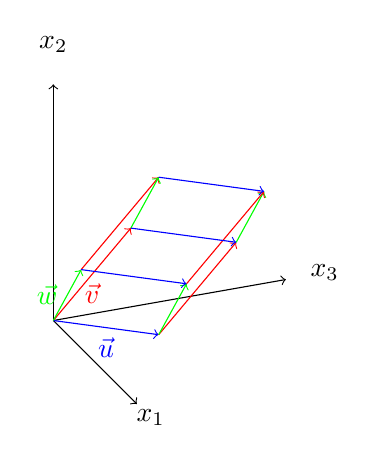
\begin{tikzpicture}
			[z={(10:10mm)},x={(-45:5mm)}]
			
			\draw[->](0,0,0) -- (xyz cylindrical cs:radius=3);
			\node at (3.5,0,0){$x_1$};
			\draw[->] (0,0,0) -- (xyz cylindrical cs:radius=3,angle=90);
			\node at (0,3.5,0){$x_2$};
			\draw[->] (0,0,0) -- (xyz cylindrical cs:z=3);
			\node at (0,0,3.5){$x_3$};
			\draw[->,color=red] 
			(0,0,0)--(0,1,1)
			node[midway, below] {\color{red}$\vec{v}$};
			\draw[->,color=blue] 
			(0,0,0)--(1,0,1)
			node[midway,below]{\color{blue}$\vec{u}$};
			\draw[->,color=green] 
			(0,0,0)--(1,1,0)
			node[midway, left]{\color{green}$\vec{w}$};
			
			\draw[->,color=red] 
			(1,0,1)--(1,1,2);
			
			\draw[->,color=green] 
			(1,1,2)--(2,2,2);
			\draw[->,color=red] 
			(1,1,0)--(1,2,1);
			\draw[->,color=green] 
			(1,0,1)--(2,1,1);
			\draw[->,color=red] (2,1,1)--(2,2,2);
			\draw[->,color=green] 
			(0,1,1)--(1,2,1);
			
			\draw[->,color=blue] 
			(1,1,0)--(2,1,1);
			
			\draw[->,color=blue] 
			(1,2,1)--(2,2,2);
			\draw[->,color=blue]
			(0,1,1)--(1,1,2);
		\end{tikzpicture}
		\caption{The parallelepiped, draw in an optical illusion fashion.}
	\end{subfigure}
	\begin{subfigure}{0.4\textwidth}
		\centering
		\begin{tikzpicture}
			[z={(10:10mm)},x={(-45:5mm)}]
			
			\draw[->](0,0,0) -- (xyz cylindrical cs:radius=3);
			\node at (3.5,0,0){$x_1$};
			\draw[->] (0,0,0) -- (xyz cylindrical cs:radius=3,angle=90);
			\node at (0,3.5,0){$x_2$};
			\draw[->] (0,0,0) -- (xyz cylindrical cs:z=3);
			\node at (0,0,3.5){$x_3$};
			\draw[->,color=red] 
			(0,0,0)--(0,1,1)
			node[midway, below] {\color{red}$\vec{v}$};
			\draw[->,color=blue] 
			(0,0,0)--(1,0,1)
			node[midway,below]{\color{blue}$\vec{u}$};
			\draw[->,color=green] 
			(0,0,0)--(1,1,0)
			node[midway, left]{\color{green}$\vec{w}$};
			\draw[->,dotted,thick]
			(0,0,0)--(-1,1,-1)
			node[midway,left]{$\vec{A}$};
			\draw[->,color=red] 
			(1,1,0)--(1,2,1);
			\draw[->,color=green] 
			(0,1,1)--(1,2,1);
			
		\end{tikzpicture}
		\caption{We want to get the projection of $\vec{u}$ on $\vec{A}$.}
	\end{subfigure}
\end{figure}\ \\
The volume is thus \[
	|\textrm{Proj}_{\vec{A}}(\vec{u})||\vec{v}|=|\frac{\vec{u}\cdot\vec{A}}{|\vec{A}|^2}|\times |\vec{A}| \times|\vec{A}| = |\vec{u}\cdot\vec{A}| = 2.
\]\ \\

\proposition{
The volume of the parallelpiped formed from $\vec{v},\vec{w},\vec{u}$ is \[
|(\vec{v}\times\vec{w})\cdot{\vec{u}}|
\]
}\ \\

\begin{remark}
	This is also the expression of the (absolute value of) determinant of \[
	\begin{bmatrix}
		\vec{v}&\vec{w}&\vec{u}
	\end{bmatrix}
	\]
	Using properties of the determinant (later chapters), you can show cycling the three vectors does not change the volume. (i.e. you can calculate using what order of the three vectors you want)
\end{remark}
	
\begin{remark}
	You may notice that the expression$(\vec{v}\times\vec{w})\cdot{\vec{u}}$ can take on negative volumes. In this case, the three vectors (taken in order) do not follow the right-hand rule. For instance, in the last example, $\vec{u}$ points in the `opposite' direction as $\vec{A}$.
\end{remark}
\exercises
\begin{exerciselist}
	\item meow
\end{exerciselist}
\section{Applications - Geometry of lines and planes}
\exercises
\begin{exerciselist}
	\item computation exercises
	\item Verify that the dot product is symmetric, linear, and positive definite.
	\item Show that $|a\vec{v}| = |a||\vec{v}|$.
\end{exerciselist}
	
	

